\documentclass[tikz,border=0pt,11pt]{standalone}
\usepackage[T1]{fontenc}
\usepackage{lmodern,amsmath,amssymb}
\usetikzlibrary{arrows.meta,calc,positioning,backgrounds}
\definecolor{blue}{HTML}{0072B2}
\definecolor{orange}{HTML}{D55E00}
\definecolor{green}{HTML}{009E73}
\definecolor{purple}{HTML}{8C5694}
\definecolor{ink}{HTML}{25313B}
\renewcommand{\familydefault}{\sfdefault}
\begin{document}
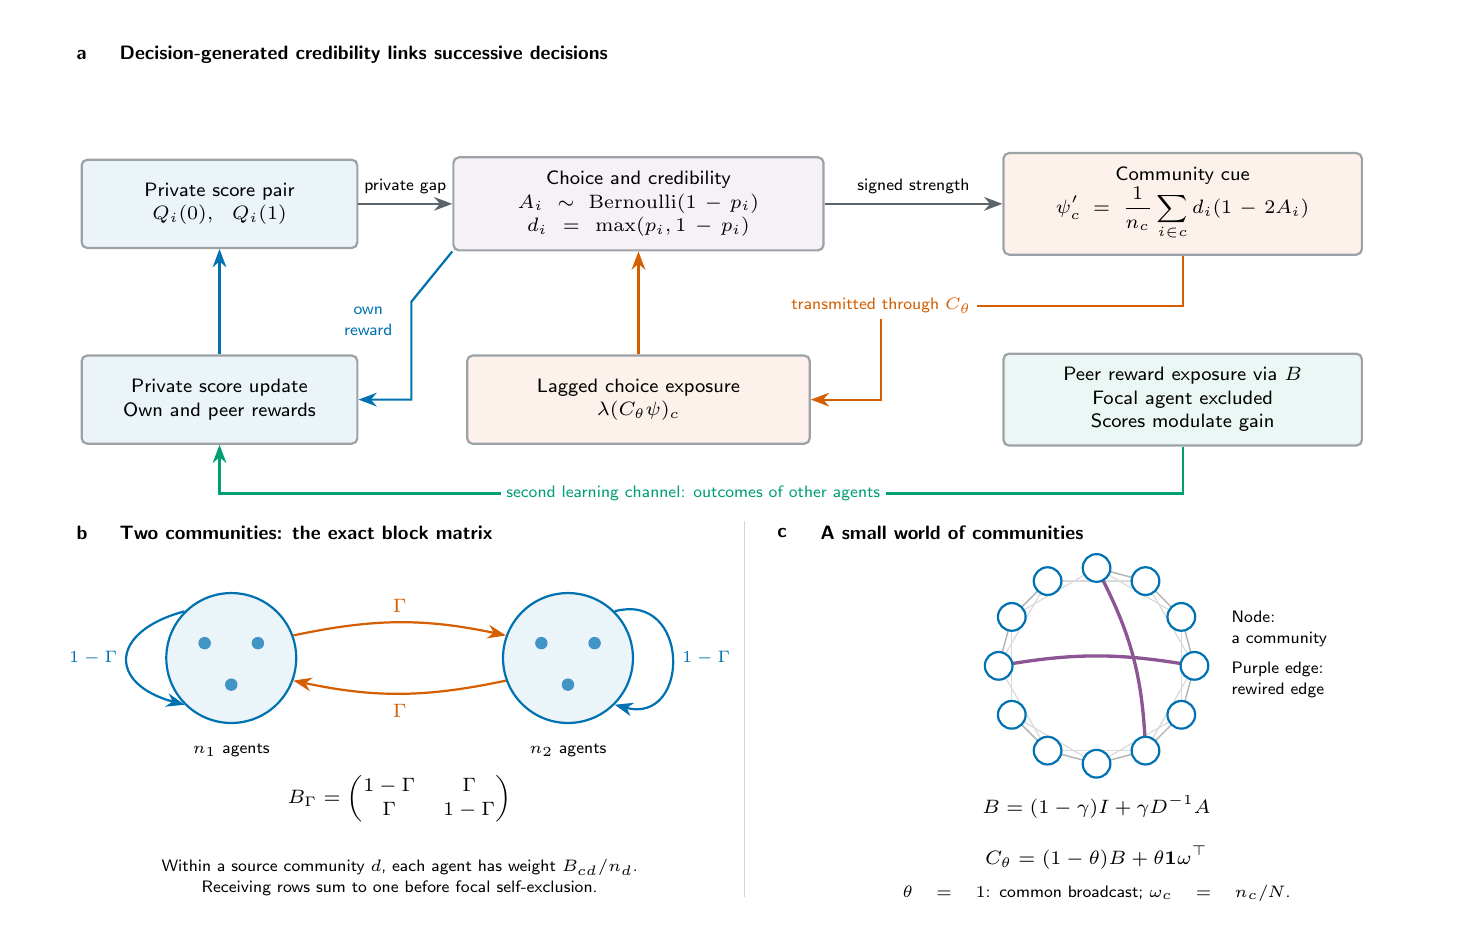
\begin{tikzpicture}[x=.994475cm,y=.994475cm,font=\sffamily\fontsize{7}{8.5}\selectfont,>=Stealth,
 box/.style={draw=ink!45,rounded corners=2pt,thick,align=center,minimum height=1.12cm,text width=3.15cm,inner sep=5pt},
 arrow/.style={->,thick,draw=ink!75},
 agent/.style={circle,fill=blue!75,inner sep=0pt,minimum size=4.5pt},
 community/.style={circle,draw=blue,fill=blue!8,thick,minimum size=1.65cm},
 meta/.style={circle,draw=blue,fill=white,thick,minimum size=10pt,inner sep=0pt}]
 \path[use as bounding box] (-.8,-.35) rectangle (17.3,10.9);
 \node[anchor=west,font=\sffamily\fontsize{7}{8.5}\selectfont\bfseries] at (-.3,10.55) {a};
 \node[anchor=west,font=\sffamily\fontsize{7}{8.5}\selectfont\bfseries] at (.25,10.55) {Decision-generated credibility links successive decisions};
 \node[box,fill=blue!8] (q) at (1.65,8.65) {Private score pair\\$Q_i(0),\;Q_i(1)$};
 \node[box,fill=purple!8,text width=4.35cm] (choice) at (7,8.65) {Choice and credibility\\$A_i\sim\mathrm{Bernoulli}(1-p_i)$\\$d_i=\max(p_i,1-p_i)$};
 \node[box,fill=orange!8,text width=4.2cm] (signal) at (13.95,8.65) {Community cue\\$\displaystyle\psi_c'=\frac{1}{n_c}\sum_{i\in c}d_i(1-2A_i)$};
 \node[box,fill=blue!8] (reward) at (1.65,6.15) {Private score update\\Own and peer rewards};
 \node[box,fill=orange!8,text width=4.0cm] (field) at (7,6.15) {Lagged choice exposure\\$\lambda(C_\theta\psi)_c$};
 \node[box,fill=green!8,text width=4.2cm] (peer) at (13.95,6.15) {Peer reward exposure via $B$\\Focal agent excluded\\Scores modulate gain};
 \draw[arrow] (q)--node[above,font=\sffamily\fontsize{6.5}{7.7}\selectfont] {private gap} (choice);
 \draw[arrow] (choice)--node[above,font=\sffamily\fontsize{6.5}{7.7}\selectfont] {signed strength} (signal);
 \draw[arrow,orange] (signal.south)--(13.95,7.35)--(10.1,7.35)--(10.1,6.15)--(field.east);
 \node[font=\sffamily\fontsize{6.5}{7.7}\selectfont,text=orange,fill=white,inner sep=2pt] at (10.1,7.35) {transmitted through $C_\theta$};
 \draw[arrow,orange] (field.north)--(choice.south);
 \draw[arrow,blue] (choice.south west)--(4.1,7.4)--(4.1,6.15)--(reward.east);
 \node[font=\sffamily\fontsize{6.5}{7.7}\selectfont,text=blue,align=center,fill=white,inner sep=2pt] at (3.55,7.15) {own\\reward};
 \draw[arrow,blue] (reward.north)--(q.south);
 \draw[arrow,green] (peer.south)--(13.95,4.95)--(1.65,4.95)--(reward.south);
 \node[font=\sffamily\fontsize{6.5}{7.7}\selectfont,text=green,fill=white,inner sep=2pt] at (7.7,4.95) {second learning channel: outcomes of other agents};
 \node[anchor=west,font=\sffamily\fontsize{7}{8.5}\selectfont\bfseries] at (-.3,4.45) {b};
 \node[anchor=west,font=\sffamily\fontsize{7}{8.5}\selectfont\bfseries] at (.25,4.45) {Two communities: the exact block matrix};
 \node[community] (c1) at (1.8,2.85) {};
 \node[community] (c2) at (6.1,2.85) {};
 \foreach \c in {c1,c2}{
  \node[agent] at ($ (\c.center)+(-.34,.19) $) {};
  \node[agent] at ($ (\c.center)+(.34,.19) $) {};
  \node[agent] at ($ (\c.center)+(0,-.34) $) {};
 }
 \node[anchor=north,font=\sffamily\fontsize{6.5}{7.7}\selectfont] at (1.8,1.88) {$n_1$ agents};
 \node[anchor=north,font=\sffamily\fontsize{6.5}{7.7}\selectfont] at (6.1,1.88) {$n_2$ agents};
 \draw[arrow,orange] (c1.20) to[bend left=12] node[above] {$\Gamma$} (c2.160);
 \draw[arrow,orange] (c2.200) to[bend left=12] node[below] {$\Gamma$} (c1.340);
 \draw[arrow,blue] (c1.135) to[loop left,min distance=10mm] node[left,font=\sffamily\fontsize{6.5}{7.7}\selectfont] {$1-\Gamma$} (c1.225);
 \draw[arrow,blue] (c2.45) to[loop right,min distance=10mm] node[right,font=\sffamily\fontsize{6.5}{7.7}\selectfont] {$1-\Gamma$} (c2.315);
 \node[align=center,font=\sffamily\fontsize{7}{8.5}\selectfont] at (3.95,1.05) {$\displaystyle B_\Gamma=\begin{pmatrix}1-\Gamma&\Gamma\\\Gamma&1-\Gamma\end{pmatrix}$};
 \node[align=center,font=\sffamily\fontsize{6.5}{7.7}\selectfont,text width=7.5cm] at (3.95,.05) {Within a source community $d$, each agent has weight $B_{cd}/n_d$.\\Receiving rows sum to one before focal self-exclusion.};
 \draw[ink!20] (8.35,-.2)--(8.35,4.6);
 \node[anchor=west,font=\sffamily\fontsize{7}{8.5}\selectfont\bfseries] at (8.65,4.45) {c};
 \node[anchor=west,font=\sffamily\fontsize{7}{8.5}\selectfont\bfseries] at (9.2,4.45) {A small world of communities};
 \foreach \i in {0,...,11}{
  \pgfmathsetmacro{\a}{90+30*\i}
  \coordinate (v\i) at ($(12.85,2.75)+(\a:1.25)$);
 }
 \foreach \i in {0,...,11}{
  \pgfmathtruncatemacro{\j}{mod(\i+1,12)}
  \pgfmathtruncatemacro{\k}{mod(\i+2,12)}
  \ifnum\i=0\else\ifnum\i=3\else
   \draw[ink!35,line width=.55pt] (v\i)--(v\j);
  \fi\fi
  \draw[ink!18,line width=.45pt] (v\i)--(v\k);
 }
 \draw[purple,very thick] (v0) to[bend left=13] (v7);
 \draw[purple,very thick] (v3) to[bend left=10] (v9);
 \foreach \i in {0,...,11}{\node[meta] at (v\i) {};}
 \node[anchor=west,align=left,font=\sffamily\fontsize{6.5}{7.7}\selectfont,text width=2.2cm] at (14.45,2.9) {Node:\\a community\\[3pt]Purple edge:\\rewired edge};
 \node[align=center,font=\sffamily\fontsize{7}{8.5}\selectfont] at (12.85,.95) {$B=(1-\gamma)I+\gamma D^{-1}A$};
 \node[align=center,font=\sffamily\fontsize{7}{8.5}\selectfont] at (12.85,.30) {$C_\theta=(1-\theta)B+\theta\mathbf1\omega^\top$};
 \node[align=center,font=\sffamily\fontsize{6.5}{7.7}\selectfont,text width=7.6cm] at (12.85,-.15) {$\theta=1$: common broadcast; $\omega_c=n_c/N$.};
\end{tikzpicture}
\end{document}
